\chapter{Forced Vibrations \& Resonance}

\fbox{
	\begin{minipage}{\linewidth}{
	\linespread{1.5}\selectfont
	
	In this chapter, we consider the effects of a \textbf{driving force} $F(t)$ on a system:
	\[ {F(t) = F_0 \cos(\omega t)} \]
	where...
	\begin{itemize}
		\item $\omega$ represents the \textbf{driving frequency}
		\item $\omega_0$ represents the \textbf{natural frequency} of the system, associated with a \textbf{free vibration} (see Chapter~\ref{ch:free-vibrations})
	\end{itemize}
	}
\end{minipage}}
\vspace{0.5em}

We will see that...
\begin{itemize}
	\item As $\omega \to \omega_0$, the amplitude of oscillation increases
	\item ... whereas as $\omega$ gets farther away from $\omega_0$, the amplitude becomes smaller
	\item This phenomenon is known as \textbf{resonance}.
\end{itemize}

The system will initially have the tendency to vibrate at $\omega_0$, but it will ultimately begin to vibrate at $\omega$. We thus have two stages:
\begin{enumerate}
	\item \textbf{Transient state}: we have a superposition of oscillations at frequencies $\omega$ and $\omega_0$. The free vibration gradually gets damped away until...
	\item \textbf{Steady state}: only the the driving vibration remains, so the system oscillates at $\omega$
\end{enumerate}

\section{Forced Oscillations without Damping}
We will consider the \emph{steady state} of a forced oscillation with negligible damping, ignoring the fact that we need damping to get past the transient state.

Force equation:
\begin{align}
	m\ddot{x} &= -kx + F_0 \cos(\omega t)  \notag \\
	\Longrightarrow
	\mcol{m}\ddot{x} + \kcol{k}x &= F_0 \cos(\omega t)	\label{ch4:eq-no-b}
\end{align}

\paragraph{Case (a): $\omega < \omega_0$}
If the driving force's frequency is much lower than the natural frequency...
\begin{itemize}
	\item We expect a low acceleration (since $\ddot{x} \propto \omega^2$).
	\item So, the $\kcol{k}x$ term dominates over $\mcol{m}\ddot{x}$.
	\item The response is controlled by the \kcol{stiffness} of the string.
	\item Since $F_0 \approx kA$, the amplitiude will be $A\approx F_0/k$
\end{itemize}

\paragraph{Case (b): $\omega > \omega_0$}
If the driving force's frequency is much higher than the natural frequency...
\begin{itemize}
	\item We expect a higher acceleration (since $\ddot{x} \propto \omega^2$).
	\item So, the $\mcol{m}\ddot{x}$ term dominates over $\kcol{k}x$.
	\item The response is controlled by the \mcol{inertia} of the string.
	\item We expect a relatively small $A$, opposite in phase with the driving force (since $x$ is 180°  out of phase from $\ddot{x}$)\footnote{Notice that in Figure~\ref{ch4:no-damping-pendula}b, when $F$ is to the left, $x$ is to the right; when $F$ is to the right, $x$ is to the left.}
\end{itemize}

These cases are summarized in Figure~\ref{ch4:no-damping-pendula}.

\begin{figure}[h]
	\centering
	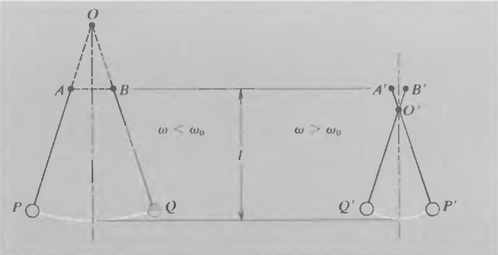
\includegraphics[scale=0.7]{phys232/Ch4-forced-no-damping-pendula.png} 
	\caption{The motion of simple pendula undergoing horizontal forced oscillations when (a) $\omega<\omega_0$ and (b) $\omega>\omega_0$.}\label{ch4:no-damping-pendula}
\end{figure}

\begin{center}
\begin{tabular}{cccc}
	\hline
	\multicolumn{2}{c}{Case} & $A$ & \parbox{3cm}{\centering Phase difference $\alpha$ b/w $x$ \& $F$}  \\
	\hline
	(a) & $\omega < \omega_0$ & large & 0° \\
	(b) & $\omega > \omega_0$ & small & 180° \\
	\hline
\end{tabular}
\end{center}


\subsection{Responant response when $\omega = \omega_0$}

We will now examine why the resonant amplitude is much greater than otherwise.

\begin{proof}[Finding the steady-state solution]
Because we are in the steady state, assume that the natural oscillations are not present:
\begin{align*}
	x &= C\cos(\omega t) \\
	\Longrightarrow
	\ddot{x} &= -\omega^2 C\cos(\omega t)
\end{align*}

Substitute this into \eqref{ch4:eq-no-b}:
\begin{align*}
	-m\omega^2 C\cancel{\cos(\omega t)} + kC\cancel{\cos(\omega t)} &= F_0\cancel {\cos(\omega t)} \\
	C(k-m\omega^2) &= F_0
\end{align*}
\begin{equation}
	 C = \frac{F_0}{k-m\omega^2} = \frac{F_0/m}{\omega_0^2-\omega^2} \label{ch4:C-no-b}
\end{equation}

\eqref{ch4:C-no-b} is plotted in Figure~\ref{ch4:no-damping-C}. Notice that as $\omega\to\omega_0$, $C\to \infty$.
\begin{figure}
	\centering
	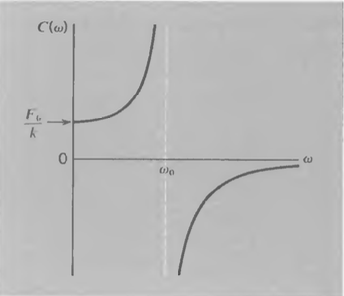
\includegraphics[scale=0.7]{phys232/Ch4-forced-no-damping-C.png} \caption{Amplitude of forced oscillations (no damping) as a function of the driving frequency $\omega$.}\label{ch4:no-damping-C}
\end{figure}

We can reexpress this solution in terms of $A=|C|$ and a value of $\alpha$ to represent the phase lag between $x$ and the driving force:
\begin{equation}
	\therefore
	x = A \cos(\omega t + \alpha)  \where \alpha = 
	\begin{cases}
		0 & \text{if } \omega<\omega_0 \\
		\pi & \text{if } \omega>\omega_0
	\end{cases}
	\label{ch4:A-no-b}
\end{equation}

\begin{figure}
	\centering
	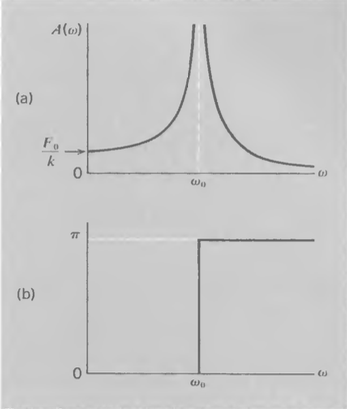
\includegraphics[scale=0.7]{phys232/Ch4-forced-no-damping-A.png} \caption{(a) Absolute amplitude of forced oscillations (no damping) as a function of $\omega$; (b) phase lag of $x$ with respect to the driving force, as a function of $\omega$.}	\label{ch4:no-damping-A}
\end{figure}

\eqref{ch4:A-no-b} is plotted in Figure~\ref{ch4:no-damping-A}.

\end{proof}

\section{Forced Oscillations with Damping}

\subsubsection{Steady State}

Equation of motion:
\[ m\ddot{x} = -kx - b\dot{x} + F_0 \cos(\omega t) \]
\[ \ddot{x} + \gamma\dot{x} + \omega_0^2 = F_0 \cos(\omega t) \]

Results: 
\[ x = A \cos (\omega t - \delta) \]
\[ A(\omega) = \frac{F_0/m}{[(\omega_0^2 - \omega^2)^2 + (\gamma\omega)^2]^{1/2}} \]
\[ \tan \delta (\omega) = \frac{\gamma\omega}{\omega_0^2 - \omega^2}\]

Independent of adjustable initial starting conditions!

\subsubsection{Transient Effects}
For $t<0$, let the object be at rest (i.e. it only starts moving at $t=0$).
\begin{align*}
x &= steady + transient \\
x &= A \cos (\omega t - \delta) + B e^{-\gamma t/2} \cos(\omega' + \beta)
\end{align*}

The transient part (system's ''natural" motion) dies out over time due to damping; after then, the steady state takes over. 

Transient part of the equation accounts for adjustable initial conditions!

A \emph{beat pattern} may be produced during this stage if $\omega'$ (system's freq w/ damping) and $\omega$ are similar.

\section{Power}
Power required to keep a driven oscillator going at the same amplitude:
\[ P = \frac{dW}{dt} = F\frac{dx}{dt} = Fv \]